\documentclass[thesis.tex]{subfiles}

\begin{document}

% ----------------------------------------------------------
\chapter{Experiments and results} \label{chap:experiments}
% ----------------------------------------------------------
% Present your results and findings
% ----------------------------------------------------------
In this section, we will first describe our experiment details. We will then present our..
Lastly, we demonstrate the surprising improvements of our models on domain specific image classification tasks with Hyper-Kvasir and Hyper-CapsuleCam datasets.



% ----------------------------------------------------------
\section{Training details}
% use this section to write about how we managed to get a good classifier
% batch_size, epoch_number, optimizer, dropout, model, image size and other hyper parameters
% ----------------------------------------------------------
% Introduction

% Batch size
For labeled images we re-scale the images to 128 by 128 pixel to reduce memory usage during training. For the smallest model, EfficientNetB0 with 4.7 million parameters, we use a batch size of 128 by default and reduce the batch size when we could not fit the model into the memory. The largest model, EfficientNetB7 with 65.4 million parameters, we reduce the batch size to 32. We find that using a batch size of 256, 128, 64 and 32 leads to the same performance as long as the dataset are resampled. When the data have dominant class imbalances the smaller batch sizes would lead to faster overfitting than the large ones.

% Epochs and training steps
We determine the number of training steps and the learning rate schedule by the batch size for labeled images. The training steps used are calculated by $$ steps = \frac{ds\_size}{bs} $$ where $ds\_size$ is the number of samples in the given train/test/val dataset and $bs$ is the value for batch size we are using. We find that the network have tendencies to overfit the training data when we use a large value for epochs (see Figure \ref{fig:overfit} for an example). Because of this we use early stopping from the tf.keras.callbacks.EarlyStopping package. This  monitors the validation loss during training, and if the model don't improve for 5 epochs the training is terminated and the epoch with the lowest loss, and therefor the best weights, is restored. Depending om model size we use, this would happen somewhere around epoch number 30. The larger model would take longer to hit early stopping threshold than the smaller ones.

\begin{figure} % fig:overfit
  \begin{center}
    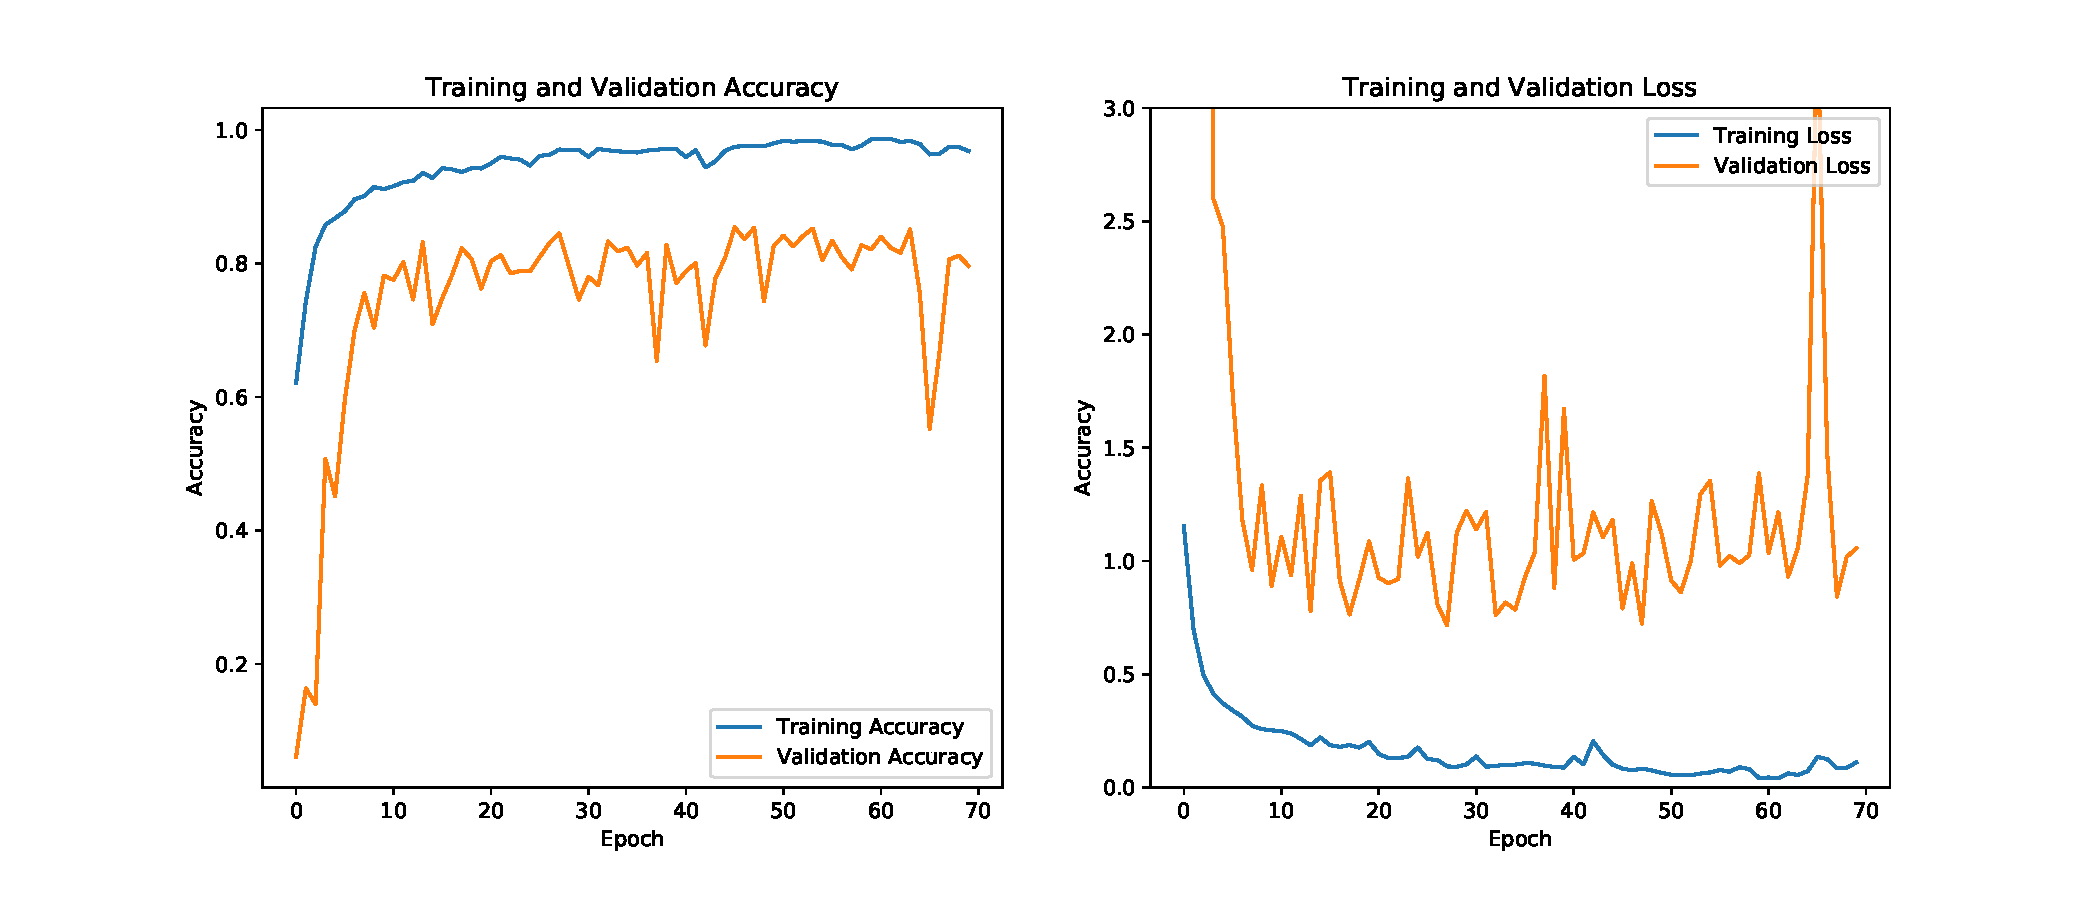
\includegraphics[width=.7\textwidth]{overfit}
    \caption[]{}
    \label{fig:overfit}
  \end{center}
\end{figure}

% Optimizer and learning rate
The optimizer we use is for our experiments are Adam \cite{AdamMethod17}, we use this optimizer because it has shown to perform well for image classification tasks in other studies. Compared to SGD algorithm we get very stable 


\subsection{Labeled and labeled dataset}
% Specify which datasets we used to run our experiments


\subsection{Architecture}




% ----------------------------------------------------------
\section{Experiments}
%
% ----------------------------------------------------------


\section{Binary vs multiclass}
% Perhaps skip if it requires to much effort and time to make data binary..
% ----------------------------------------------------------



\subsection{Weight initialization}
% initializing the model with weights vs without weigts.
% initializing the student with the teacher model's weights?
% mention imagenet weights are trained using autoAugment
% ----------------------------------------------------------
Found that training on Hyper-Kvasir datasets yield best results when using EfficientNet with is initialized with weights from ImageNet. Early in our study the only pre-trained weights readily available were trained without the use of AutoAugment, and performed slightly worse than the ImageNet weights trained with AutoAugment, released at a later time. Especially we observed that the model would initialize the training with lower loss when trained with ImageNet-AutoAugment weigths.

%TODO insert plot of training loss and accuracy (and class-report?) of imagenet-autoaugment and imagenet

We tested with initializing the teacher model with original noisy-student weights but found that loss were fluxing more early in training. Also when trained for same number of epochs as with ImageNet weights the model would perform worse on the evaluation data, with lower accuracy and lower recall.

%TODO insert plot of training loss and accuracy (and class-report?) of noisy-student

As part of this experiment we also tested with initializing the teacher model with no weights and train from scratch. Not surprisingly, this gave slower training, and after 20 epochs we got a 15\% lower accuracy than when training with ImageNet weights.



\subsection{Class Weigting vs Resample}
Found that by re-sampling the dataset the model generelized much better than by calculating the loss from weighted class distribution.




\subsection{Model complexity}
% how model size effects how the teacher model learns






% ----------------------------------------------------------
\section{Teacher-student model}
% section for everything teacher-student
% ----------------------------------------------------------



\subsection{Noising the student}



\subsection{Model size}
% Test how model size effects the performance of teacher/student model
% a; small model vs large model
% b; iterative larger model during training
% ----------------------------------------------------------





\subsection{Number of iterations}
% how many iterations of swapping student with teacher to get good results?
% ----------------------------------------------------------





% ----------------------------------------------------------
\section{Results} \label{sec:C4-results}
% ----------------------------------------------------------






% ----------------------------------------------------------
\section{Summary} \label{sec:C4-summary}
% ----------------------------------------------------------




\end{document}